\documentclass[a4paper,10pt]{article}
%
\usepackage{amsmath}
\usepackage{graphicx}
\usepackage{hyperref}
\usepackage{url}
%
\newcommand{\cH}{\mathcal{H}}
\newcommand{\cJ}{\mathcal{J}}
\newcommand{\cS}{\mathcal{S}}
\newcommand{\cZ}{\mathcal{Z}}
%
\begin{document}
%
\title{SHHEIG Users' Guide}
\author{
Peter Benner\thanks{Max Planck Institute for Dynamics of Complex Technical Systems, Sandtorstra{\ss}e 1, 39016 Magdeburg, Germany, e-mail: \texttt{benner@mpi-magdeburg.mpg.de}},
Vasile Sima\thanks{National Institute for Research \& Development in Informatics (ICI), Lab. 07, 8--10 Averescu Ave., Bucharest 1, Romania, code 011455, e-mail: \texttt{vsima@ici.ro}}, and
Matthias Voigt\thanks{Technische Universit\"at Berlin, Sekretariat MA 4-5, Stra{\ss}e des 17. Juni 136, 10623 Berlin, Germany, e-mail: \texttt{mvoigt@math.tu-berlin.de}}
}
%
\maketitle
%
\begin{abstract}
SHHEIG is a software package for solving of skew-Hamiltonian/Ha\-miltonian eigenproblems using structure-preserving algorithms. In this users' guide we give an overview of this software and hints on its installation and usage.
\end{abstract}
%
\section{Introduction}
%
SHHEIG is a Fortran 77 software package for the solution of generalized eigenvalue problems for $2n \times 2n$ skew-Hamiltonian/Hamiltonian matrix pencils $\lambda \cS - \cH$. This package provides implementations of structure-preserving algorithms to 
\begin{itemize}
 \item compute the eigenvalues;
 \item reorder the eigenvalues in the computed structured normal forms;
 \item compute the stable deflating subspaces, i.e., the deflating subspaces to the eigenvalues with negative real part.
\end{itemize}
For these tasks there exist subroutines for dealing with problems where the skew-Hamiltonian matrix $\cS$ is explicitly given, and for problems where only the factor $\cZ$ of 
\begin{equation*}
 \cS = \cJ \cZ^H \cJ^T \cZ \quad \text{with} \quad \cJ = \begin{bmatrix} 0 & I_n \\ -I_n & 0 \end{bmatrix}
\end{equation*}
is known. Moreover, all subroutines have versions to deal with real and complex data, respectively. In order to exploit the cache more efficiently for larger problems, SHHEIG contains blocked versions of the codes (for explicitly given $\cS$ only). For a detailed derivation of the algorithms we refer to \cite{BenBMX01,BenBLMX07}. For details on the implementation and numerical examples we refer to \cite{BenSV14}.
\section{Contents}
The SHHEIG package is distributed via an archive \texttt{shheig.tar.gz}. After extraction one obtains the SHHEIG root directory \texttt{shheig}
containing the following directories and files:
\begin{itemize}
 \item the directory \texttt{src}, containing the Fortran 77 source files;
 \item the directory \texttt{examples}, containing Fortran test programs (\texttt{*.f}) and corresponding data input files (\texttt{*.dat}) and example output files (\texttt{*.res});
 \item the directory \texttt{doc}, containing the html documentation describing input and output parameters as well as example inputs and outputs of the Fortran routines in \texttt{src};
 \item the directory \texttt{mex}, containing MEX-files (\texttt{*.F}) for generating gateway functions that can be used to call the Fortran routines in MATLAB;
 \item the directory \texttt{test}, containing MATLAB functions for testing the functionality and performance of the gateway functions generated by the MEX-files included in \texttt{mex},
 \item the directory \texttt{usersguide}, containing this users' guide;
 \item a \texttt{makefile} and the file \texttt{make.inc} for building the SHHEIG library;
 \item the documentation index \texttt{libindex.html}.
 \item a \texttt{readme} file containing some general hints.
\end{itemize}
%
\section{Installation and Usage}
%
\subsection{Before Installation}
%
SHHEIG routines make calls to subprograms from the state-of-the-art packages SLICOT (Subroutine Library in Control Theory), LAPACK (Linear 
Algebra Package) and BLAS (Basic Linear Algebra Subprograms). Thus it is necessary to download and install these libraries before building the SHHEIG library.

SLICOT source code and the prebuilt library is freely available for academic users after registration from the SLICOT website (\url{http://slicot.org}). The LAPACK and BLAS libraries are freely downloadable from netlib (\url{http://www.netlib.org/}). However, for maximum efficiency it is recommended to use machine-specific, optimized versions whenever possible.
%
\subsection{Building the SHHEIG Library}
%
Template make files are provided to help building the SHHEIG Library object files, and to link and run the available example programs calling
the SHHEIG Library routines. In order to use these make files on a specific Unix platform, some changes might be needed in the files 
\texttt{make.inc} and/or \texttt{makefile} stored in the SHHEIG root directory.

The changes in \texttt{make.inc} might define the specific machine (platform) identifier, the compiler, linker, and archiver flags, as well as the location and names of the SLICOT, LAPACK, and BLAS libraries, which the program files should be linked to. Details are given in the file \texttt{make.inc}.

\textbf{IMPORTANT:} On 64bit platforms the code must be compiled with the options \texttt{-fPIC} and \texttt{-fdefault-integer-8}, for instance by setting
\begin{verbatim}
   OPTS = -O2 -fPIC -fdefault-integer-8
\end{verbatim}
in \texttt{make.inc}.

Changes in the makefile might be needed for using a Fortran 77 compiler, since a Fortran 90/95 compiler is assumed by default to build the
executable example programs. (The SHHEIG routines themselves are written in Fortran 77.)

After performing the necessary changes, as suggested in the comments of the make files, the other needed SHHEIG-related files can be generated
automatically with the command
\begin{verbatim}
   make
\end{verbatim}
issued from the SHHEIG root directory \texttt{shheig}.

The first execution of \texttt{make} will create the following files:
\begin{itemize}
 \item the SHHEIG library object files \texttt{*.o} in the subdirectory \texttt{src} of \texttt{shheig};
 \item the library file \texttt{shheig.a}, in the directory \texttt{shheig};
 \item the example program object and executable files, in the subdirectory \texttt{examples};
 \item the files \texttt{*.exa}, with the results computed on the local machine, with the same names as the files with data (\texttt{*.dat}) and reference results (\texttt{*.res}), also in the subdirectory \texttt{examples}.
\end{itemize}
  
The subsequent executions of make will update the files if changes have been performed.

The files \texttt{*.exa}, with the computed results may be compared with the reference results. Several types of differences could be noticed,
including possible sign changes for some elements, or even different values in some columns and/or rows of the computed matrices. For 
instance, the matrices of similarity or equivalence transformations could differ from a platform/compiler to another. This does not usually mean 
that the computed results are wrong.

More details for executing other tasks, e.g., cleaning the subdirectories \texttt{src} and \texttt{examples}, are given in the files \texttt{makefile} included in the directory \texttt{shheig} and in the subdirectories \texttt{src} and \texttt{examples}.
%
\subsection{Creating Gateway Functions for Running SHHEIG in MATLAB}
%
For ease of usage, MEX-files contained in the subdirectory \texttt{mex} have been written to generate gateway functions that allow the user the call the main subroutines in MATLAB. There are two ways to compile the MEX-files.

The easiest way consists of going to the subdirectory \texttt{mex} and typing the command
\begin{verbatim}
   allmex
\end{verbatim}
in MATLAB. This command will first call the MATLAB functions \texttt{slicotmex} and \texttt{shheigmex} that generate the SLICOT and SHHEIG libraries using the built-in Fortran compiler of MATLAB. The respective library files are called \texttt{mexslicot.a} and \texttt{mexshheig.a}. Then the function \texttt{makemex} generates the gateway functions from the MEX-files which will then be tested by the function \texttt{testmex}. The functions called by \texttt{allmex} detect which kind of machine is used and will automatically set the correct flags. However, depending on the location of the SLICOT source files, it might be necessary to modify the value of the variable \texttt{slicot\_src} in \texttt{slicotmex.m}, or alternatively, use the path of the SLICOT source files as an argument in \texttt{allmex}.

The second method consists of linking the SLICOT and SHHEIG library files generated outside of MATLAB when compiling the MEX-files. To do so it is necessary to modify the values of the variables \texttt{libslicot} and \texttt{libshheig} in the file \texttt{makemex.m}. Then the gateway functions are generated by typing
\begin{verbatim}
   makemex
\end{verbatim}
and tested by typing 
\begin{verbatim}
   testmex
\end{verbatim}
in MATLAB in the subdirectory \texttt{mex}.
%
\bibliographystyle{plain}
\bibliography{refs}
%
\appendix
%
\section{Interfaces and Call Graphs of the Driver Routines}
%
\subsection{The Subroutine \texttt{DGHFDF}}
%
\footnotesize
\begin{verbatim}
      SUBROUTINE DGHFDF( COMPQ, COMPU, ORTH, N, Z, LDZ, B, LDB, FG,
     $                   LDFG, NEIG, Q, LDQ, U, LDU, ALPHAR, ALPHAI,
     $                   BETA, IWORK, LIWORK, DWORK, LDWORK, BWORK,
     $                   IWARN, INFO )
C
C     PURPOSE
C
C     To compute the relevant eigenvalues of a real N-by-N skew-
C     Hamiltonian/Hamiltonian pencil aS - bH, with
C
C                                   (  B  F  )      (  0  I  )
C       S = T Z = J Z' J' Z and H = (        ), J = (        ),      (1)
C                                   (  G -B' )      ( -I  0  )
C
C     where the notation M' denotes the transpose of the matrix M.
C     Optionally, if COMPQ = 'C', an orthogonal basis of the right
C     deflating subspace of aS - bH corresponding to the eigenvalues
C     with strictly negative real part is computed. Optionally, if
C     COMPU = 'C', an orthonormal basis of the companion subspace,
C     range(P_U) [1], which corresponds to the eigenvalues with strictly
C     negative real part, is computed.
C
C     ARGUMENTS
C
C     Mode Parameters
C
C     COMPQ   CHARACTER*1
C             Specifies whether to compute the right deflating subspace
C             corresponding to the eigenvalues of aS - bH with strictly
C             negative real part.
C             = 'N':  do not compute the deflating subspace;
C             = 'C':  compute the deflating subspace and store it in the
C                     leading subarray of Q.
C
C     COMPU   CHARACTER*1
C             Specifies whether to compute the companion subspace
C             corresponding to the eigenvalues of aS - bH with strictly
C             negative real part.
C             = 'N': do not compute the companion subspace;
C             = 'C': compute the companion subspace and store it in the
C                    leading subarray of U.
C
C     ORTH    CHARACTER*1
C             If COMPQ = 'C' and/or COMPU = 'C', specifies the technique
C             for computing the orthogonal basis of the deflating
C             subspace, and/or of the companion subspace, as follows:
C             = 'P':  QR factorization with column pivoting;
C             = 'S':  singular value decomposition.
C             If COMPQ = 'N' and COMPU = 'N', the ORTH value is not
C             used.
C
C     Input/Output Parameters
C
C     N       (input) INTEGER
C             The order of the pencil aS - bH.  N >= 0, even.
C
C     Z       (input/output) DOUBLE PRECISION array, dimension (LDZ, N)
C             On entry, the leading N-by-N part of this array must
C             contain the non-trivial factor Z in the factorization
C             S = J Z' J' Z of the skew-Hamiltonian matrix S.
C             On exit, if COMPQ = 'C' or COMPU = 'C', the leading
C             N-by-N part of this array contains the transformed upper
C                               ~
C             triangular matrix Z11 (see METHOD), after moving the
C             eigenvalues with strictly negative real part to the top
C             of the pencil (3). The strictly lower triangular part is
C             not zeroed.
C             If COMPQ = 'N' and COMPU = 'N', the leading N-by-N part of
C             this array contains the matrix Z obtained by the routine
C             DGHURV just before the application of the periodic QZ
C             algorithm. The elements of the (2,1) block, i.e., in the
C             rows N/2+1 to N and in the columns 1 to N/2 are not set to
C             zero, but are unchanged on exit.
C
C     LDZ     INTEGER
C             The leading dimension of the array Z.  LDZ >= MAX(1, N).
C
C     B       (input) DOUBLE PRECISION array, dimension (LDB, N/2)
C             On entry, the leading N/2-by-N/2 part of this array must
C             contain the matrix B.
C
C     LDB     INTEGER
C             The leading dimension of the array B.  LDB >= MAX(1, N/2).
C
C     FG      (input) DOUBLE PRECISION array, dimension (LDFG, N/2+1)
C             On entry, the leading N/2-by-N/2 lower triangular part of
C             this array must contain the lower triangular part of the
C             symmetric matrix G, and the N/2-by-N/2 upper triangular
C             part of the submatrix in the columns 2 to N/2+1 of this
C             array must contain the upper triangular part of the
C             symmetric matrix F.
C
C     LDFG    INTEGER
C             The leading dimension of the array FG.
C             LDFG >= MAX(1, N/2).
C
C     NEIG    (output) INTEGER
C             If COMPQ = 'C' or COMPU = 'C', the number of eigenvalues
C             in aS - bH with strictly negative real part.
C
C     Q       (output) DOUBLE PRECISION array, dimension (LDQ, 2*N)
C             On exit, if COMPQ = 'C', the leading N-by-NEIG part of
C             this array contains an orthogonal basis of the right
C             deflating subspace corresponding to the eigenvalues of
C             aS - bH with strictly negative real part. The remaining
C             part of this array is used as workspace.
C             If COMPQ = 'N', this array is not referenced.
C
C     LDQ     INTEGER
C             The leading dimension of the array Q.
C             LDQ >= 1,           if COMPQ = 'N';
C             LDQ >= MAX(1, 2*N), if COMPQ = 'C'.
C
C     U       (output) DOUBLE PRECISION array, dimension (LDU, 2*N)
C             On exit, if COMPU = 'C', the leading N-by-NEIG part of
C             this array contains an orthogonal basis of the companion
C             subspace corresponding to the eigenvalues of aS - bH with
C             strictly negative real part. The remaining part of this
C             array is used as workspace.
C             If COMPU = 'N', this array is not referenced.
C
C     LDU     INTEGER
C             The leading dimension of the array U.
C             LDU >= 1,         if COMPU = 'N';
C             LDU >= MAX(1, N), if COMPU = 'C'.
C
C     ALPHAR  (output) DOUBLE PRECISION array, dimension (N/2)
C             The real parts of each scalar alpha defining an eigenvalue
C             of the pencil aS - bH.
C
C     ALPHAI  (output) DOUBLE PRECISION array, dimension (N/2)
C             The imaginary parts of each scalar alpha defining an
C             eigenvalue of the pencil aS - bH.
C             If ALPHAI(j) is zero, then the j-th eigenvalue is real.
C
C     BETA    (output) DOUBLE PRECISION array, dimension (N/2)
C             The scalars beta that define the eigenvalues of the pencil
C             aS - bH.
C             If INFO = 0, the quantities alpha = (ALPHAR(j),ALPHAI(j)),
C             and beta = BETA(j) represent together the j-th eigenvalue
C             of the pencil aS - bH, in the form lambda = alpha/beta.
C             Since lambda may overflow, the ratios should not, in
C             general, be computed. Due to the skew-Hamiltonian/
C             Hamiltonian structure of the pencil, only half of the
C             spectrum is saved in ALPHAR, ALPHAI and BETA.
C             Specifically, only eigenvalues with imaginary parts
C             greater than or equal to zero are stored; their conjugate
C             eigenvalues are not stored. If imaginary parts are zero
C             (i.e., for real eigenvalues), only positive eigenvalues
C             are stored. The remaining eigenvalues have opposite signs.
C             If IWARN = 1, one or more BETA(j) is not representable,
C             and the eigenvalues are returned as described below (see
C             the description of the argument IWARN).
C
C     Workspace
C
C     IWORK   INTEGER array, dimension (LIWORK)
C             On exit, if INFO = -20, IWORK(1) returns the minimum value
C             of LIWORK.
C             On exit, if INFO = 0 and IWARN = 1, then IWORK(1), ...,
C             IWORK(N/2) return the scaling parameters for the
C             eigenvalues of the pencil aS - bH (see IWARN).
C
C     LIWORK  INTEGER
C             The dimension of the array IWORK.
C             LIWORK >= N + 18,      if COMPQ = 'N' and COMPU = 'N';
C             LIWORK >= MAX( N + 18, N/2 + 48, 5*N/2 + 1 ), otherwise.
C
C     DWORK   DOUBLE PRECISION array, dimension (LDWORK)
C             On exit, if INFO = 0, DWORK(1) returns the optimal value
C             of LDWORK, and DWORK(2) returns the machine base, b.
C             On exit, if INFO = -22, DWORK(1) returns the minimum value
C             of LDWORK.
C
C     LDWORK  INTEGER
C             The dimension of the array DWORK.
C             LDWORK >= c*N**2 + max( N*N + MAX( N/2+252, 432 ),
C                                     MAX(8*N+48,171) ), where
C                       c = a,   if COMPU = 'N',
C                       c = a+1, if COMPU = 'C', and
C                       a = 6,   if COMPQ = 'N',
C                       a = 9,   if COMPQ = 'C'.
C             For good performance LDWORK should be generally larger.
C
C             If LDWORK = -1  a workspace query is assumed; the
C             routine only calculates the optimal size of the DWORK
C             array, returns this value as the first entry of the DWORK
C             array, and no error message is issued by XERBLA.
C
C     BWORK   LOGICAL array, dimension (N/2)
C
C     Warning Indicator
C
C     IWARN   INTEGER
C             = 0: no warning;
C             = 1: the eigenvalues will under- or overflow if evaluated;
C                  therefore, the j-th eigenvalue is represented by
C                  the quantities alpha = (ALPHAR(j),ALPHAI(j)),
C                  beta = BETA(j), and gamma = IWORK(j) in the form
C                  lambda = (alpha/beta) * b**gamma, where b is the
C                  machine base (often 2.0), returned in DWORK(2).
C
C     Error Indicator
C
C     INFO    INTEGER
C             = 0: succesful exit;
C             < 0: if INFO = -i, the i-th argument had an illegal value;
C             = 1: periodic QZ iteration failed in the routines DGHURV,
C                  DGHFYR or the SLICOT libaray routine MB03BB (QZ
C                  iteration did not converge or computation of the
C                  shifts failed);
C             = 2: standard QZ iteration failed in the routines DGHFYR
C                  or DGHFEX (called by DGHFXC);
C             = 3: a numerically singular matrix was found in the routine
C                  DGHFEY (called by DGHFXC);
C             = 4: the singular value decomposition failed in the LAPACK
C                  routine DGESVD (for ORTH = 'S').
C
C     METHOD
C
C     First, the decompositions of S and H are computed via orthogonal
C     matrices Q1 and Q2 and orthogonal symplectic matrices U1 and U2,
C     such that
C
C                                   ( T11  T12 )
C       Q1' T U1 = Q1' J Z' J' U1 = (          ),
C                                   (  0   T22 )
C
C                  ( Z11  Z12 )
C       U2' Z Q2 = (          ),                                     (2)
C                  (  0   Z22 )
C
C                  ( H11  H12 )
C       Q1' H Q2 = (          ),
C                  (  0   H22 )
C
C     where T11, T22', Z11, Z22', H11 are upper triangular and H22' is
C     upper quasi-triangular.
C
C     Then, orthogonal matrices Q3, Q4 and U3 are found, for the
C     matrices
C
C       ~     ( T22'  0  )  ~     ( T11'  0  )  ~   (   0   H11 )
C       Z11 = (          ), Z22 = (          ), H = (           ),
C             (  0   Z11 )        (  0   Z22 )      ( -H22'  0  )
C
C               ~          ~       ~          ~
C     such that Z11 := U3' Z11 Q4, Z22 := U3' Z22 Q3 are upper
C                    ~          ~
C     triangular and H11 := Q3' H Q4 is upper quasi-triangular. The
C     following matrices are computed:
C
C       ~          ( -T12'  0  )        ~          (  0   H12 )
C       Z12 := U3' (           ) Q3 and H12 := Q3' (          ) Q3.
C                  (  0    Z12 )                   ( H12'  0  )
C
C     Then, an orthogonal matrix Q and an orthogonal symplectic matrix U
C     are found such that the eigenvalues with strictly negative real
C     parts of the pencil
C
C             ~    ~          ~    ~           ~    ~
C           ( Z11  Z12 )'   ( Z11  Z12 )     ( H11  H12  )
C       a J (      ~   ) J' (      ~   ) - b (      ~    )           (3)
C           (  0   Z22 )    (  0   Z22 )     (  0  -H11' )
C
C     are moved to the top of this pencil.
C
C     Finally, an orthogonal basis of the right deflating subspace
C     and an orthogonal basis of the companion subspace corresponding to
C     the eigenvalues with strictly negative real part are computed.
C     See also page 11 in [1] for more details.
C
C     REFERENCES
C
C     [1] Benner, P., Byers, R., Losse, P., Mehrmann, V. and Xu, H.
C         Numerical Solution of Real Skew-Hamiltonian/Hamiltonian
C         Eigenproblems.
C         Tech. Rep., Technical University Chemnitz, Germany,
C         Nov. 2007.
C
C     NUMERICAL ASPECTS
C                                                               3
C     The algorithm is numerically backward stable and needs O(N )
C     floating point operations.
C
C     FURTHER COMMENTS
C
C     This routine does not perform any scaling of the matrices. Scaling
C     might sometimes be useful, and it should be done externally.
\end{verbatim}
%
\begin{figure}[ht]
 \centering
 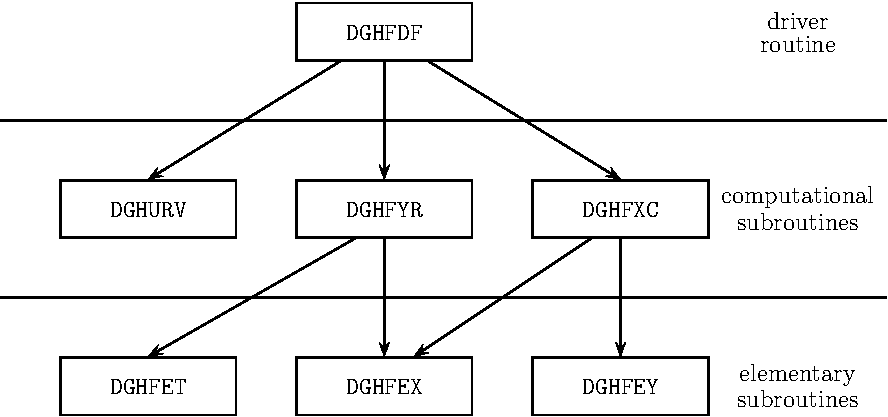
\includegraphics[width=0.8\textwidth]{real_factored.pdf}
 \caption{Call graph of DGHFDF.}
\end{figure}
%
\subsection{The Subroutine \texttt{DGHUDF}}
%
\begin{verbatim}
      SUBROUTINE DGHUDF( COMPQ, ORTH, N, A, LDA, DE, LDDE, B, LDB, FG,
     $                   LDFG, NEIG, Q, LDQ, ALPHAR, ALPHAI, BETA,
     $                   IWORK, LIWORK, DWORK, LDWORK, BWORK, INFO )
C
C     PURPOSE
C
C     To compute the relevant eigenvalues of a real N-by-N skew-
C     Hamiltonian/Hamiltonian pencil aS - bH, with
C
C           (  A  D  )         (  B  F  )
C       S = (        ) and H = (        ),                           (1)
C           (  E  A' )         (  G -B' )
C
C     where the notation M' denotes the transpose of the matrix M.
C     Optionally, if COMPQ = 'C', an orthogonal basis of the right
C     deflating subspace of aS - bH corresponding to the eigenvalues
C     with strictly negative real part is computed.
C
C     ARGUMENTS
C
C     Mode Parameters
C
C     COMPQ   CHARACTER*1
C             Specifies whether to compute the right deflating subspace
C             corresponding to the eigenvalues of aS - bH with strictly
C             negative real part.
C             = 'N':  do not compute the deflating subspace;
C             = 'C':  compute the deflating subspace and store it in the
C                     leading subarray of Q.
C
C     ORTH    CHARACTER*1
C             If COMPQ = 'C', specifies the technique for computing the
C             orthogonal basis of the deflating subspace, as follows:
C             = 'P':  QR factorization with column pivoting;
C             = 'S':  singular value decomposition.
C             If COMPQ = 'N', the ORTH value is not used.
C
C     Input/Output Parameters
C
C     N       (input) INTEGER
C             The order of the pencil aS - bH.  N >= 0, even.
C
C     A       (input/output) DOUBLE PRECISION array, dimension
C                            (LDA, N/2)
C             On entry, the leading N/2-by-N/2 part of this array must
C             contain the matrix A.
C             On exit, if COMPQ = 'C', the leading N/2-by-N/2 part of
C             this array contains the upper triangular matrix Aout
C             (see METHOD); otherwise, it contains the upper triangular
C             matrix A obtained just before the application of the
C             periodic QZ algorithm (see the routine DGHUTR).
C
C     LDA     INTEGER
C             The leading dimension of the array A.  LDA >= MAX(1, N/2).
C
C     DE      (input/output) DOUBLE PRECISION array, dimension
C                            (LDDE, N/2+1)
C             On entry, the leading N/2-by-N/2 lower triangular part of
C             this array must contain the lower triangular part of the
C             skew-symmetric matrix E, and the N/2-by-N/2 upper
C             triangular part of the submatrix in the columns 2 to N/2+1
C             of this array must contain the upper triangular part of the
C             skew-symmetric matrix D.
C             The entries on the diagonal and the first superdiagonal of
C             this array need not be set, but are assumed to be zero.
C             On exit, if COMPQ = 'C', the leading N/2-by-N/2 lower
C             triangular part and the first superdiagonal contain the
C             transpose of the upper quasi-triangular matrix C2out (see
C             METHOD), and the (N/2-1)-by-(N/2-1) upper triangular part
C             of the submatrix in the columns 3 to N/2+1 of this array
C             contains the strictly upper triangular part of the
C             skew-symmetric matrix Dout (see METHOD), without the main
C             diagonal, which is zero.
C             On exit, if COMPQ = 'N', the leading N/2-by-N/2 lower
C             triangular part and the first superdiagonal contain the
C             transpose of the upper Hessenberg matrix C2, and the
C             (N/2-1)-by-(N/2-1) upper triangular part of the submatrix
C             in the columns 3 to N/2+1 of this array contains the
C             strictly upper triangular part of the skew-symmetric
C             matrix D (without the main diagonal) just before the
C             application of the periodic QZ algorithm.
C
C     LDDE    INTEGER
C             The leading dimension of the array DE.
C             LDDE >= MAX(1, N/2).
C
C     B       (input/output) DOUBLE PRECISION array, dimension
C                            (LDB, N/2)
C             On entry, the leading N/2-by-N/2 part of this array must
C             contain the matrix B.
C             On exit, if COMPQ = 'C', the leading N/2-by-N/2 part of
C             this array contains the upper triangular matrix C1out
C             (see METHOD); otherwise, it contains the upper triangular
C             matrix C1 obtained just before the application of the
C             periodic QZ algorithm.
C
C     LDB     INTEGER
C             The leading dimension of the array B.  LDB >= MAX(1, N/2).
C
C     FG      (input/output) DOUBLE PRECISION array, dimension
C                            (LDFG, N/2+1)
C             On entry, the leading N/2-by-N/2 lower triangular part of
C             this array must contain the lower triangular part of the
C             symmetric matrix G, and the N/2-by-N/2 upper triangular
C             part of the submatrix in the columns 2 to N/2+1 of this
C             array must contain the upper triangular part of the
C             symmetric matrix F.
C             On exit, if COMPQ = 'C', the leading N/2-by-N/2 part of
C             the submatrix in the columns 2 to N/2+1 of this array
C             contains the matrix Vout (see METHOD); otherwise, it
C             contains the matrix V obtained just before the application
C             of the periodic QZ algorithm.
C
C     LDFG    INTEGER
C             The leading dimension of the array FG.
C             LDFG >= MAX(1, N/2).
C
C     NEIG    (output) INTEGER
C             If COMPQ = 'C', the number of eigenvalues in aS - bH with
C             strictly negative real part.
C
C     Q       (output) DOUBLE PRECISION array, dimension (LDQ, 2*N)
C             On exit, if COMPQ = 'C', the leading N-by-NEIG part of
C             this array contains an orthogonal basis of the right
C             deflating subspace corresponding to the eigenvalues of
C             aA - bB with strictly negative real part. The remaining
C             part of this array is used as workspace.
C             If COMPQ = 'N', this array is not referenced.
C
C     LDQ     INTEGER
C             The leading dimension of the array Q.
C             LDQ >= 1,           if COMPQ = 'N';
C             LDQ >= MAX(1, 2*N), if COMPQ = 'C'.
C
C     ALPHAR  (output) DOUBLE PRECISION array, dimension (N/2)
C             The real parts of each scalar alpha defining an eigenvalue
C             of the pencil aS - bH.
C
C     ALPHAI  (output) DOUBLE PRECISION array, dimension (N/2)
C             The imaginary parts of each scalar alpha defining an
C             eigenvalue of the pencil aS - bH.
C             If ALPHAI(j) is zero, then the j-th eigenvalue is real.
C
C     BETA    (output) DOUBLE PRECISION array, dimension (N/2)
C             The scalars beta that define the eigenvalues of the pencil
C             aS - bH.
C             Together, the quantities alpha = (ALPHAR(j),ALPHAI(j)) and
C             beta = BETA(j) represent the j-th eigenvalue of the pencil
C             aS - bH, in the form lambda = alpha/beta. Since lambda may
C             overflow, the ratios should not, in general, be computed.
C             Due to the skew-Hamiltonian/Hamiltonian structure of the
C             pencil, for every eigenvalue lambda, -lambda is also an
C             eigenvalue, and thus it has only to be saved once in
C             ALPHAR, ALPHAI and BETA.
C             Specifically, only eigenvalues with imaginary parts
C             greater than or equal to zero are stored; their conjugate
C             eigenvalues are not stored. If imaginary parts are zero
C             (i.e., for real eigenvalues), only positive eigenvalues
C             are stored. The remaining eigenvalues have opposite signs.
C
C     Workspace
C
C     IWORK   INTEGER array, dimension (LIWORK)
C             On exit, if INFO = -19, IWORK(1) returns the minimum value
C             of LIWORK.
C
C     LIWORK  INTEGER
C             The dimension of the array IWORK.
C             LIWORK >= MAX( 32, N + 12, 2*N + 1 ).
C
C     DWORK   DOUBLE PRECISION array, dimension (LDWORK)
C             On exit, if INFO = 0, DWORK(1) returns the optimal LDWORK.
C             On exit, if INFO = -21, DWORK(1) returns the minimum value
C             of LDWORK.
C
C     LDWORK  INTEGER
C             The dimension of the array DWORK.
C             LDWORK >= 3*(N/2)**2 + N**2 + MAX( MAX( N, 32 ) + 4,
C                                             4*(N+1) ), if COMPQ = 'N',
C               where the last term can be reduced to 4*N if N/2 is odd;
C             LDWORK >= 8*N**2 + MAX( 8*N + 32, N/2 + 168, 272 ),
C                                                        if COMPQ = 'C'.
C             For good performance LDWORK should be generally larger.
C
C             If LDWORK = -1  a workspace query is assumed; the
C             routine only calculates the optimal size of the DWORK
C             array, returns this value as the first entry of the DWORK
C             array, and no error message is issued by XERBLA.
C
C     BWORK   LOGICAL array, dimension (N/2)
C
C     Error Indicator
C
C     INFO    INTEGER
C             = 0: succesful exit;
C             < 0: if INFO = -i, the i-th argument had an illegal value;
C             = 1: periodic QZ iteration failed in the routines DGHUTR or
C                  DGHUYR (QZ iteration did not converge or computation
C                  of the shifts failed);
C             = 2: standard QZ iteration failed in the routines DGHUYR or
C                  DGHUEX (called by DGHUXC);
C             = 3: a numerically singular matrix was found in the routine
C                  DGHUEY (called by DGHUXC);
C             = 4: the singular value decomposition failed in the LAPACK
C                  routine DGESVD (for ORTH = 'S').
C
C     METHOD
C
C     First, the decompositions of S and H are computed via orthogonal
C     transformations Q1 and Q2 as follows:
C
C                       (  Aout  Dout  )
C       Q1' S J Q1 J' = (              ),
C                       (   0    Aout' )
C
C                       (  Bout  Fout  )
C       J' Q2' J S Q2 = (              ) =: T,                       (2)
C                       (   0    Bout' )
C
C                  (  C1out  Vout  )            (  0  I  )
C       Q1' H Q2 = (               ), where J = (        ),
C                  (  0     C2out' )            ( -I  0  )
C
C     and Aout, Bout, C1out are upper triangular, C2out is upper quasi-
C     triangular and Dout and Fout are skew-symmetric.
C
C     Then, orthogonal matrices Q3 and Q4 are found, for the extended
C     matrices
C
C            (  Aout   0  )          (    0   C1out )
C       Se = (            ) and He = (              ),
C            (   0   Bout )          ( -C2out   0   )
C
C     such that S11 := Q4' Se Q3 is upper triangular and
C     H11 := Q4' He Q3 is upper quasi-triangular. The following matrices
C     are computed:
C
C                  (  Dout   0  )                   (   0   Vout )
C       S12 := Q4' (            ) Q4 and H12 := Q4' (            ) Q4.
C                  (   0   Fout )                   ( Vout'   0  )
C
C     Then, an orthogonal matrix Q is found such that the eigenvalues
C     with strictly negative real parts of the pencil
C
C         (  S11  S12  )     (  H11  H12  )
C       a (            ) - b (            )
C         (   0   S11' )     (   0  -H11' )
C
C     are moved to the top of this pencil.
C
C     Finally, an orthogonal basis of the right deflating subspace
C     corresponding to the eigenvalues with strictly negative real part
C     is computed. See also page 12 in [1] for more details.
C
C     REFERENCES
C
C     [1] Benner, P., Byers, R., Losse, P., Mehrmann, V. and Xu, H.
C         Numerical Solution of Real Skew-Hamiltonian/Hamiltonian
C         Eigenproblems.
C         Tech. Rep., Technical University Chemnitz, Germany,
C         Nov. 2007.
C
C     NUMERICAL ASPECTS
C                                                               3
C     The algorithm is numerically backward stable and needs O(N )
C     floating point operations.
C
C     FURTHER COMMENTS
C
C     This routine does not perform any scaling of the matrices. Scaling
C     might sometimes be useful, and it should be done externally.
\end{verbatim}
%
\begin{figure}[ht]
 \centering
 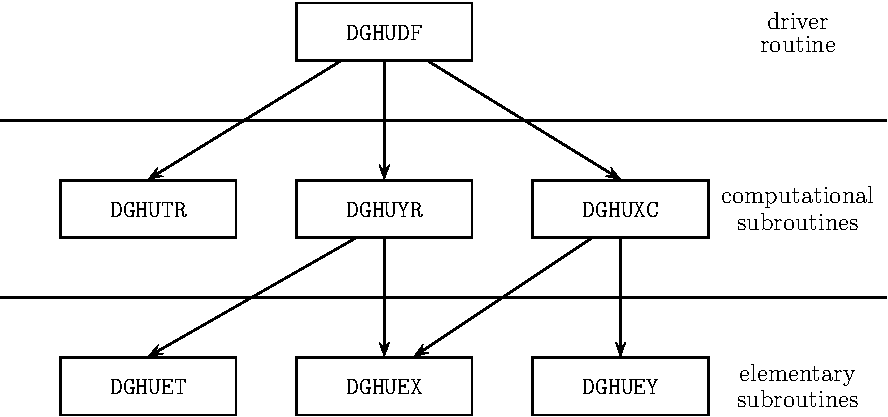
\includegraphics[width=0.8\textwidth]{real_unfactored.pdf}
 \caption{Call graph of DGHUDF.}
\end{figure}
%
\subsection{The Subroutine \texttt{ZGHFDF}}
%
\begin{verbatim}
      SUBROUTINE ZGHFDF( COMPQ, COMPU, ORTH, N, Z, LDZ, B, LDB, FG,
     $                   LDFG, NEIG, D, LDD, C, LDC, Q, LDQ, U, LDU,
     $                   ALPHAR, ALPHAI, BETA, IWORK, LIWORK, DWORK,
     $                   LDWORK, ZWORK, LZWORK, BWORK, INFO )
C
C     PURPOSE
C
C     To compute the eigenvalues of a complex N-by-N skew-Hamiltonian/
C     Hamiltonian pencil aS - bH, with
C
C                             (  B  F  )      (  Z11  Z12  )
C       S = J Z' J' Z and H = (        ), Z = (            ),
C                             (  G -B' )      (  Z21  Z22  )
C                                                                   (1)
C           (  0  I  )
C       J = (        ).
C           ( -I  0  )
C
C     The structured Schur form of the embedded real skew-Hamiltonian/
C                                                            
C     skew-Hamiltonian pencil, aB_S - bB_T, with B_S = J B_Z' J' B_Z,
C
C             (  Re(Z11)  -Im(Z11)  |  Re(Z12)  -Im(Z12)  )
C             (                     |                     )
C             (  Im(Z11)   Re(Z11)  |  Im(Z12)   Re(Z12)  )
C             (                     |                     )
C       B_Z = (---------------------+---------------------) ,
C             (                     |                     )
C             (  Re(Z21)  -Im(Z21)  |  Re(Z22)  -Im(Z22)  )
C             (                     |                     )
C             (  Im(Z21)   Re(Z21)  |  Im(Z22)   Re(Z22)  )
C                                                                    (2)
C             ( -Im(B)  -Re(B)  | -Im(F)  -Re(F)  )
C             (                 |                 )
C             (  Re(B)  -Im(B)  |  Re(F)  -Im(F)  )
C             (                 |                 )
C       B_T = (-----------------+-----------------) ,  T = i*H,
C             (                 |                 )
C             ( -Im(G)  -Re(G)  | -Im(B')  Re(B') )
C             (                 |                 )
C             (  Re(G)  -Im(G)  | -Re(B') -Im(B') )
C
C     is determined and used to compute the eigenvalues. Optionally, if
C     COMPQ = 'C', an orthonormal basis of the right deflating subspace,
C     Def_-(S, H), of the pencil aS - bH in (1), corresponding to the
C     eigenvalues with strictly negative real part, is computed. Namely,
C     after transforming aB_S - bB_H, in the factored form, by unitary
C     matrices, we have B_Sout = J B_Zout' J' B_Zout,
C
C                ( BA  BD  )              ( BB  BF  )
C       B_Zout = (         ) and B_Hout = (         ),               (3)
C                (  0  BC  )              (  0 -BB' )
C
C     and the eigenvalues with strictly negative real part of the
C     complex pencil aB_Sout - bB_Hout are moved to the top. The 
C     notation M' denotes the conjugate transpose of the matrix M.
C     Optionally, if COMPU = 'C', an orthonormal basis of the companion
C     subspace, range(P_U) [1], which corresponds to the eigenvalues
C     with negative real part, is computed. The embedding doubles the
C     multiplicities of the eigenvalues of the pencil aS - bH.
C
C     ARGUMENTS
C
C     Mode Parameters
C
C     COMPQ   CHARACTER*1
C             Specifies whether to compute the right deflating subspace
C             corresponding to the eigenvalues of aS - bH with strictly
C             negative real part.
C             = 'N': do not compute the deflating subspace;
C             = 'C': compute the deflating subspace and store it in the
C                    leading subarray of Q.
C
C     COMPU   CHARACTER*1
C             Specifies whether to compute the companion subspace
C             corresponding to the eigenvalues of aS - bH with strictly
C             negative real part.
C             = 'N': do not compute the companion subspace;
C             = 'C': compute the companion subspace and store it in the
C                    leading subarray of U.
C
C     ORTH    CHARACTER*1
C             If COMPQ = 'C' or COMPU = 'C', specifies the technique for
C             computing the orthonormal bases of the deflating subspace
C             and companion subspace, as follows:
C             = 'P':  QR factorization with column pivoting;
C             = 'S':  singular value decomposition.
C             If COMPQ = 'N' and COMPU = 'N', the ORTH value is not
C             used.
C
C     Input/Output Parameters
C
C     N       (input) INTEGER
C             Order of the pencil aS - bH.  N >= 0, even.
C
C     Z       (input/output) COMPLEX*16 array, dimension (LDZ, N)
C             On entry, the leading N-by-N part of this array must
C             contain the non-trivial factor Z in the factorization
C             S = J Z' J' Z of the skew-Hamiltonian matrix S.
C             On exit, if COMPQ = 'C' or COMPU = 'C', the leading
C             N-by-N part of this array contains the upper triangular
C             matrix BA in (3) (see also METHOD). The strictly lower
C             triangular part is not zeroed.
C             If COMPQ = 'N' and COMPU = 'N', this array is unchanged
C             on exit.
C
C     LDZ     INTEGER
C             The leading dimension of the array Z.  LDZ >= MAX(1, N).
C
C     B       (input/output) COMPLEX*16 array, dimension (LDB, N)
C             On entry, the leading N/2-by-N/2 part of this array must
C             contain the matrix B.
C             On exit, if COMPQ = 'C' or COMPU = 'C', the leading
C             N-by-N part of this array contains the upper triangular
C             matrix BB in (3) (see also METHOD). The strictly lower
C             triangular part is not zeroed. 
C             If COMPQ = 'N' and COMPU = 'N', this array is unchanged
C             on exit.
C
C     LDB     INTEGER
C             The leading dimension of the array B.  LDB >= MAX(1, N).
C
C     FG      (input/output) COMPLEX*16 array, dimension (LDFG, N)
C             On entry, the leading N/2-by-N/2 lower triangular part of
C             this array must contain the lower triangular part of the
C             Hermitian matrix G, and the N/2-by-N/2 upper triangular
C             part of the submatrix in the columns 2 to N/2+1 of this
C             array must contain the upper triangular part of the
C             Hermitian matrix F.
C             On exit, if COMPQ = 'C' or COMPU = 'C', the leading
C             N-by-N part of this array contains the Hermitian matrix
C             BF in (3) (see also METHOD). The strictly lower triangular
C             part of the input matrix is preserved. The diagonal
C             elements might have tiny imaginary parts.
C             If COMPQ = 'N' and COMPU = 'N', this array is unchanged
C             on exit.
C
C     LDFG    INTEGER
C             The leading dimension of the array FG.  LDFG >= MAX(1, N).
C
C     NEIG    (output) INTEGER
C             If COMPQ = 'C' or COMPU = 'C', the number of eigenvalues
C             in aS - bH with strictly negative real part.
C
C     D       (output) COMPLEX*16 array, dimension (LDD, N)
C             If COMPQ = 'C' or COMPU = 'C', the leading N-by-N part of
C             this array contains the matrix BD in (3) (see METHOD).
C             If COMPQ = 'N' and COMPU = 'N', this array is not
C             referenced.
C
C     LDD     INTEGER
C             The leading dimension of the array D.
C             LDD >= 1,         if COMPQ = 'N' and COMPU = 'N';
C             LDD >= MAX(1, N), if COMPQ = 'C' or  COMPU = 'C'.
C
C     C       (output) COMPLEX*16 array, dimension (LDC, N)
C             If COMPQ = 'C' or COMPU = 'C', the leading N-by-N part of
C             this array contains the lower triangular matrix BC in (3)
C             (see also METHOD). The strictly upper triangular part is
C             not zeroed. 
C             If COMPQ = 'N' and COMPU = 'N', this array is not
C             referenced.
C
C     LDC     INTEGER
C             The leading dimension of the array C.
C             LDC >= 1,         if COMPQ = 'N' and COMPU = 'N';
C             LDC >= MAX(1, N), if COMPQ = 'C' or  COMPU = 'C'.
C
C     Q       (output) COMPLEX*16 array, dimension (LDQ, 2*N)
C             On exit, if COMPQ = 'C', the leading N-by-NEIG part of
C             this array contains an orthonormal basis of the right
C             deflating subspace corresponding to the eigenvalues of the
C             pencil aS - bH with strictly negative real part.
C             The remaining entries are meaningless.
C             If COMPQ = 'N', this array is not referenced.
C
C     LDQ     INTEGER
C             The leading dimension of the array Q.
C             LDQ >= 1,           if COMPQ = 'N';
C             LDQ >= MAX(1, 2*N), if COMPQ = 'C'.
C
C     U       (output) COMPLEX*16 array, dimension (LDU, 2*N)
C             On exit, if COMPU = 'C', the leading N-by-NEIG part of
C             this array contains an orthonormal basis of the companion
C             subspace corresponding to the eigenvalues of the
C             pencil aS - bH with strictly negative real part. The
C             remaining entries are meaningless.
C             If COMPU = 'N', this array is not referenced.
C
C     LDU     INTEGER
C             The leading dimension of the array U.
C             LDU >= 1,         if COMPU = 'N';
C             LDU >= MAX(1, N), if COMPU = 'C'.
C
C     ALPHAR  (output) DOUBLE PRECISION array, dimension (N)
C             The real parts of each scalar alpha defining an eigenvalue
C             of the pencil aS - bH.
C
C     ALPHAI  (output) DOUBLE PRECISION array, dimension (N)
C             The imaginary parts of each scalar alpha defining an
C             eigenvalue of the pencil aS - bH.
C             If ALPHAI(j) is zero, then the j-th eigenvalue is real.
C
C     BETA    (output) DOUBLE PRECISION array, dimension (N)
C             The scalars beta that define the eigenvalues of the pencil
C             aS - bH.
C             Together, the quantities alpha = (ALPHAR(j),ALPHAI(j)) and
C             beta = BETA(j) represent the j-th eigenvalue of the pencil
C             aS - bH, in the form lambda = alpha/beta. Since lambda may
C             overflow, the ratios should not, in general, be computed.
C
C     Workspace
C
C     IWORK   INTEGER array, dimension (LIWORK)
C
C     LIWORK  INTEGER
C             The dimension of the array IWORK.  LIWORK >= 2*N+9.
C
C     DWORK   DOUBLE PRECISION array, dimension (LDWORK)
C             On exit, if INFO = 0, DWORK(1) returns the optimal LDWORK.
C             On exit, if INFO = -26, DWORK(1) returns the minimum
C             value of LDWORK.
C
C     LDWORK  INTEGER
C             The dimension of the array DWORK.
C             LDWORK >= c*N**2 + N + MAX(2*N, 24) + 3, where
C                       c = 18, if                 COMPU = 'C';
C                       c = 16, if COMPQ = 'C' and COMPU = 'N';
C                       c = 13, if COMPQ = 'N' and COMPU = 'N'.
C             For good performance LDWORK should be generally larger.
C
C             If LDWORK = -1, then a workspace query is assumed;
C             the routine only calculates the optimal size of the
C             DWORK array, returns this value as the first entry of
C             the DWORK array, and no error message related to LDWORK
C             is issued by XERBLA.
C
C     ZWORK   COMPLEX*16 array, dimension (LZWORK)
C             On exit, if INFO = 0, ZWORK(1) returns the optimal LZWORK.
C             On exit, if INFO = -28, ZWORK(1) returns the minimum
C             value of LZWORK.
C
C     LZWORK  INTEGER
C             The dimension of the array ZWORK.
C             LZWORK >= 8*N + 28, if COMPQ = 'C';
C             LZWORK >= 6*N + 28, if COMPQ = 'N' and COMPU = 'C';
C             LZWORK >= 1,        if COMPQ = 'N' and COMPU = 'N'.
C             For good performance LZWORK should be generally larger.
C
C             If LZWORK = -1, then a workspace query is assumed;
C             the routine only calculates the optimal size of the
C             ZWORK array, returns this value as the first entry of
C             the ZWORK array, and no error message related to LZWORK
C             is issued by XERBLA.
C
C     BWORK   LOGICAL array, dimension (LBWORK)
C             LBWORK >= 0, if COMPQ = 'N' and COMPU = 'N';
C             LBWORK >= N, if COMPQ = 'C' or  COMPU = 'C'.
C
C     Error Indicator
C
C     INFO    INTEGER
C             = 0: succesful exit;
C             < 0: if INFO = -i, the i-th argument had an illegal value;
C             = 1: the algorithm was not able to reveal information
C                  about the eigenvalues from the 2-by-2 blocks in the
C                  SLICOT Library routine MB03BD (called by DGHFST);
C             = 2: periodic QZ iteration failed in the SLICOT Library
C                  routines MB03BD or MB03BZ when trying to
C                  triangularize the 2-by-2 blocks;
C             = 3: the singular value decomposition failed in the LAPACK
C                  routine ZGESVD (for ORTH = 'S').
C
C     METHOD
C
C     First T = i*H is set. Then, the embeddings, B_Z and B_T, of the
C     matrices S and T, are determined and, subsequently, the routine
C     DGHFST is applied to compute the structured Schur form, i.e.,
C     the factorizations
C
C     ~                (  BZ11  BZ12  )
C     B_Z = U' B_Z Q = (              ) and
C                      (    0   BZ22  )
C
C     ~                     (  T11  T12  )
C     B_T = J Q' J' B_T Q = (            ),
C                           (   0   T11' )
C
C     where Q is real orthogonal, U is real orthogonal symplectic, BZ11,
C     BZ22' are upper triangular and T11 is upper quasi-triangular.
C
C     Second, the routine ZGHFXC is applied, to compute a
C                    ~                                 ~
C     unitary matrix Q and a unitary symplectic matrix U, such that
C
C                   ~    ~
C     ~  ~   ~   (  Z11  Z12  )
C     U' B_Z Q = (       ~    ) =: B_Zout,
C                (   0   Z22  )
C
C       ~        ~    ~   (  H11  H12  )
C     J Q' J'(-i*B_T) Q = (            ) =: B_Hout,
C                         (   0  -H11' )
C          ~    ~   
C     with Z11, Z22', H11 upper triangular, and such that the spectrum
C
C              ~       ~       ~
C     Spec_-(J B_Z' J' B_Z, -i*B_T) is contained in the spectrum of the
C                                                   ~    ~
C     2*NEIG-by-2*NEIG leading principal subpencil aZ22'*Z11 - bH11.
C
C     Finally, the right deflating subspace and the companion subspace
C     are computed. See also page 21 in [1] for more details.
C
C     REFERENCES
C
C     [1] Benner, P., Byers, R., Mehrmann, V. and Xu, H.
C         Numerical Computation of Deflating Subspaces of Embedded
C         Hamiltonian Pencils.
C         Tech. Rep. SFB393/99-15, Technical University Chemnitz,
C         Germany, June 1999.
C
C     NUMERICAL ASPECTS
C                                                               3
C     The algorithm is numerically backward stable and needs O(N )
C     complex floating point operations.
C
C     FURTHER COMMENTS
C
C     This routine does not perform any scaling of the matrices. Scaling
C     might sometimes be useful, and it should be done externally.
\end{verbatim}
%
\begin{figure}[ht]
 \centering
 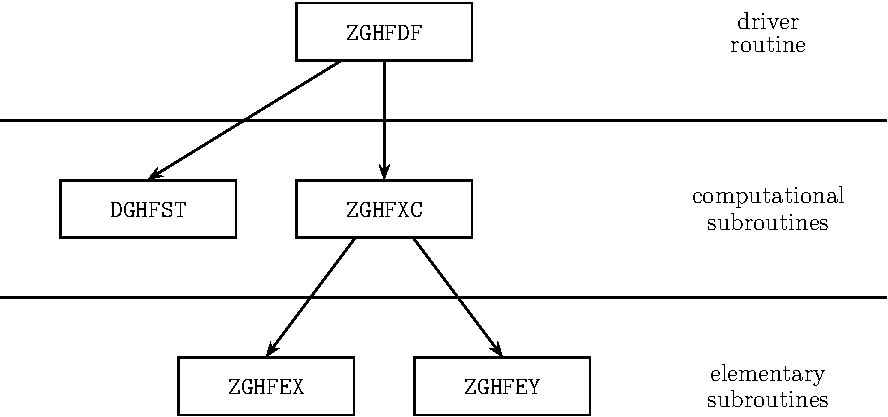
\includegraphics[width=0.8\textwidth]{complex_factored.pdf}
 \caption{Call graph of ZGHFDF.}
\end{figure}
%
\subsection{The Subroutine \texttt{ZGHUDF}}
%
\begin{verbatim}
      SUBROUTINE ZGHUDF( COMPQ, ORTH, N, A, LDA, DE, LDDE, B, LDB, FG,
     $                   LDFG, NEIG, Q, LDQ, ALPHAR, ALPHAI, BETA,
     $                   IWORK, DWORK, LDWORK, ZWORK, LZWORK, BWORK,
     $                   INFO )
C
C     PURPOSE
C
C     To compute the eigenvalues of a complex N-by-N skew-Hamiltonian/
C     Hamiltonian pencil aS - bH, with
C
C           (  A  D  )         (  B  F  )
C       S = (        ) and H = (        ).                           (1)
C           (  E  A' )         (  G -B' )
C
C     The structured Schur form of the embedded real skew-Hamiltonian/
C     skew-Hamiltonian pencil aB_S - bB_T, defined as
C
C
C             (  Re(A)  -Im(A)  |  Re(D)  -Im(D)  )
C             (                 |                 )
C             (  Im(A)   Re(A)  |  Im(D)   Re(D)  )
C             (                 |                 )
C       B_S = (-----------------+-----------------) , and
C             (                 |                 )
C             (  Re(E)  -Im(E)  |  Re(A')  Im(A') )
C             (                 |                 )
C             (  Im(E)   Re(E)  | -Im(A')  Re(A') )
C                                                                    (2)
C             ( -Im(B)  -Re(B)  | -Im(F)  -Re(F)  )
C             (                 |                 )
C             (  Re(B)  -Im(B)  |  Re(F)  -Im(F)  )
C             (                 |                 )
C       B_T = (-----------------+-----------------) ,  T = i*H,
C             (                 |                 )
C             ( -Im(G)  -Re(G)  | -Im(B')  Re(B') )
C             (                 |                 )
C             (  Re(G)  -Im(G)  | -Re(B') -Im(B') )
C
C     is determined and used to compute the eigenvalues. The notation M'
C     denotes the conjugate transpose of the matrix M. Optionally,
C     if COMPQ = 'C', an orthonormal basis of the right deflating
C     subspace of the pencil aS - bH, corresponding to the eigenvalues
C     with strictly negative real part, is computed. Namely, after
C     transforming aB_S - bB_H by unitary matrices, we have
C
C                ( BA  BD  )              ( BB  BF  )
C       B_Sout = (         ) and B_Hout = (         ),               (3)
C                (  0  BA' )              (  0 -BB' )
C
C     and the eigenvalues with strictly negative real part of the
C     complex pencil aB_Sout - bB_Hout are moved to the top. The
C     embedding doubles the multiplicities of the eigenvalues of the
C     pencil aS - bH.
C
C     ARGUMENTS
C
C     Mode Parameters
C
C     COMPQ   CHARACTER*1
C             Specifies whether to compute the deflating subspace
C             corresponding to the eigenvalues of aS - bH with strictly
C             negative real part.
C             = 'N': do not compute the deflating subspace; compute the
C                    eigenvalues only;
C             = 'C': compute the deflating subspace and store it in the
C                    leading subarray of Q.
C
C     ORTH    CHARACTER*1
C             If COMPQ = 'C', specifies the technique for computing an
C             orthonormal basis of the deflating subspace, as follows:
C             = 'P':  QR factorization with column pivoting;
C             = 'S':  singular value decomposition.
C             If COMPQ = 'N', the ORTH value is not used.
C
C     Input/Output Parameters
C
C     N       (input) INTEGER
C             The order of the pencil aS - bH.  N >= 0, even.
C
C     A       (input/output) COMPLEX*16 array, dimension (LDA, N)
C             On entry, the leading N/2-by-N/2 part of this array must
C             contain the matrix A.
C             On exit, if COMPQ = 'C', the leading N-by-N part of this
C             array contains the upper triangular matrix BA in (3) (see
C             also METHOD). The strictly lower triangular part is not
C             zeroed; it is preserved in the leading N/2-by-N/2 part.
C             If COMPQ = 'N', this array is unchanged on exit.
C
C     LDA     INTEGER
C             The leading dimension of the array A.  LDA >= MAX(1, N).
C
C     DE      (input/output) COMPLEX*16 array, dimension (LDDE, N)
C             On entry, the leading N/2-by-N/2 lower triangular part of
C             this array must contain the lower triangular part of the
C             skew-Hermitian matrix E, and the N/2-by-N/2 upper
C             triangular part of the submatrix in the columns 2 to N/2+1
C             of this array must contain the upper triangular part of
C             the skew-Hermitian matrix D.
C             On exit, if COMPQ = 'C', the leading N-by-N part of this
C             array contains the skew-Hermitian matrix BD in (3) (see
C             also METHOD). The strictly lower triangular part of the
C             input matrix is preserved.
C             If COMPQ = 'N', this array is unchanged on exit.
C
C     LDDE    INTEGER
C             The leading dimension of the array DE.  LDDE >= MAX(1, N).
C
C     B       (input/output) COMPLEX*16 array, dimension (LDB, N)
C             On entry, the leading N/2-by-N/2 part of this array must
C             contain the matrix B.
C             On exit, if COMPQ = 'C', the leading N-by-N part of this
C             array contains the upper triangular matrix BB in (3) (see
C             also METHOD). The strictly lower triangular part is not
C             zeroed; the elements below the first subdiagonal of the
C             input matrix are preserved.
C             If COMPQ = 'N', this array is unchanged on exit.
C
C     LDB     INTEGER
C             The leading dimension of the array B.  LDB >= MAX(1, N).
C
C     FG      (input/output) COMPLEX*16 array, dimension (LDFG, N)
C             On entry, the leading N/2-by-N/2 lower triangular part of
C             this array must contain the lower triangular part of the
C             Hermitian matrix G, and the N/2-by-N/2 upper triangular
C             part of the submatrix in the columns 2 to N/2+1 of this
C             array must contain the upper triangular part of the
C             Hermitian matrix F.
C             On exit, if COMPQ = 'C', the leading N-by-N part of this
C             array contains the Hermitian matrix BF in (3) (see also
C             METHOD). The strictly lower triangular part of the input
C             matrix is preserved. The diagonal elements might have tiny
C             imaginary parts.
C             If COMPQ = 'N', this array is unchanged on exit.
C
C     LDFG    INTEGER
C             The leading dimension of the array FG.  LDFG >= MAX(1, N).
C
C     NEIG    (output) INTEGER
C             If COMPQ = 'C', the number of eigenvalues in aS - bH with
C
C     Q       (output) COMPLEX*16 array, dimension (LDQ, 2*N)
C             On exit, if COMPQ = 'C', the leading N-by-NEIG part of
C             this array contains an orthonormal basis of the right
C             deflating subspace corresponding to the eigenvalues of the
C             pencil aS - bH with strictly negative real part.
C             The remaining entries are meaningless.
C             If COMPQ = 'N', this array is not referenced.
C
C     LDQ     INTEGER
C             The leading dimension of the array Q.
C             LDQ >= 1,           if COMPQ = 'N';
C             LDQ >= MAX(1, 2*N), if COMPQ = 'C'.
C
C     ALPHAR  (output) DOUBLE PRECISION array, dimension (N)
C             The real parts of each scalar alpha defining an eigenvalue
C             of the pencil aS - bH.
C
C     ALPHAI  (output) DOUBLE PRECISION array, dimension (N)
C             The imaginary parts of each scalar alpha defining an
C             eigenvalue of the pencil aS - bH.
C             If ALPHAI(j) is zero, then the j-th eigenvalue is real.
C
C     BETA    (output) DOUBLE PRECISION array, dimension (N)
C             The scalars beta that define the eigenvalues of the pencil
C             aS - bH.
C             Together, the quantities alpha = (ALPHAR(j),ALPHAI(j)) and
C             beta = BETA(j) represent the j-th eigenvalue of the pencil
C             aS - bH, in the form lambda = alpha/beta. Since lambda may
C             overflow, the ratios should not, in general, be computed.
C
C     Workspace
C
C     IWORK   INTEGER array, dimension (LIWORK)
C             LIWORK >= N, if ORTH =  'P';
C             LIWORK >= 0, if ORTH <> 'P'.
C
C     DWORK   DOUBLE PRECISION array, dimension (LDWORK)
C             On exit, if INFO = 0, DWORK(1) returns the optimal LDWORK.
C             On exit, if INFO = -20, DWORK(1) returns the minimum value
C             of LDWORK.
C
C     LDWORK  INTEGER
C             The dimension of the array DWORK.
C             LDWORK >= MAX( 1,  5*N*N + 3*N ), if COMPQ = 'N';
C             LDWORK >= MAX( 1, 11*N*N + 2*N ), if COMPQ = 'C'.
C             For good performance LDWORK should be generally larger.
C
C             If LDWORK = -1, then a workspace query is assumed;
C             the routine only calculates the optimal size of the
C             DWORK array, returns this value as the first entry of
C             the DWORK array, and no error message related to LDWORK
C             is issued by XERBLA.
C
C     ZWORK   COMPLEX*16 array, dimension (LZWORK)
C             On exit, if INFO = 0, ZWORK(1) returns the optimal LZWORK.
C             On exit, if INFO = -22, ZWORK(1) returns the minimum
C             value of LZWORK.
C
C     LZWORK  INTEGER
C             The dimension of the array ZWORK.
C             LZWORK >= 1,       if COMPQ = 'N';
C             LZWORK >= 8*N + 4, if COMPQ = 'C'.
C             For good performance LZWORK should be generally larger.
C
C             If LZWORK = -1, then a workspace query is assumed;
C             the routine only calculates the optimal size of the
C             ZWORK array, returns this value as the first entry of
C             the ZWORK array, and no error message related to LZWORK
C             is issued by XERBLA.
C
C     BWORK   LOGICAL array, dimension (LBWORK)
C             LBWORK >= 0, if COMPQ = 'N';
C             LBWORK >= N, if COMPQ = 'C'.
C
C     Error Indicator
C
C     INFO    INTEGER
C             = 0: succesful exit;
C             < 0: if INFO = -i, the i-th argument had an illegal value;
C             = 1: QZ iteration failed in the routine DGHUST (QZ
C                  iteration did not converge or computation of the
C                  shifts failed);
C             = 2: QZ iteration failed in the LAPACK routine ZHGEQZ when
C                  trying to triangularize the 2-by-2 blocks;
C             = 3: the singular value decomposition failed in the LAPACK
C                  routine ZGESVD (for ORTH = 'S').
C
C     METHOD
C
C     First, T = i*H is set. Then, the embeddings, B_S and B_T, of the
C     matrices S and T, are determined and, subsequently, the routine
C     DGHUST is applied to compute the structured Schur form, i.e., the
C     factorizations
C
C     ~                     (  S11  S12  )
C     B_S = J Q' J' B_S Q = (            ) and
C                           (   0   S11' )
C
C     ~                     (  T11  T12  )           (  0  I  )
C     B_T = J Q' J' B_T Q = (            ), with J = (        ),
C                           (   0   T11' )           ( -I  0  )
C
C     where Q is real orthogonal, S11 is upper triangular, and T11 is
C     upper quasi-triangular.
C
C     Second, the routine ZGHUXC is applied, to compute a unitary matrix
C     ~
C     Q, such that
C
C                        ~    ~
C       ~     ~   ~   (  S11  S12  )
C     J Q' J' B_S Q = (       ~    ) =: B_Sout,
C                     (   0   S11' )
C
C       ~        ~    ~   (  H11  H12  )
C     J Q' J'(-i*B_T) Q = (            ) =: B_Hout,
C                         (   0  -H11' )
C          ~                                               ~       ~
C     with S11, H11 upper triangular, and such that Spec_-(B_S, -i*B_T)
C     is contained in the spectrum of the 2*NEIG-by-2*NEIG leading
C                          ~
C     principal subpencil aS11 - bH11.
C
C     Finally, the right deflating subspace is computed.
C     See also page 22 in [1] for more details.
C
C     REFERENCES
C
C     [1] Benner, P., Byers, R., Mehrmann, V. and Xu, H.
C         Numerical Computation of Deflating Subspaces of Embedded
C         Hamiltonian Pencils.
C         Tech. Rep. SFB393/99-15, Technical University Chemnitz,
C         Germany, June 1999.
C
C     NUMERICAL ASPECTS
C                                                               3
C     The algorithm is numerically backward stable and needs O(N )
C     complex floating point operations.
C
C     FURTHER COMMENTS
C
C     This routine does not perform any scaling of the matrices. Scaling
C     might sometimes be useful, and it should be done externally.
\end{verbatim}
%
\begin{figure}[ht]
 \centering
 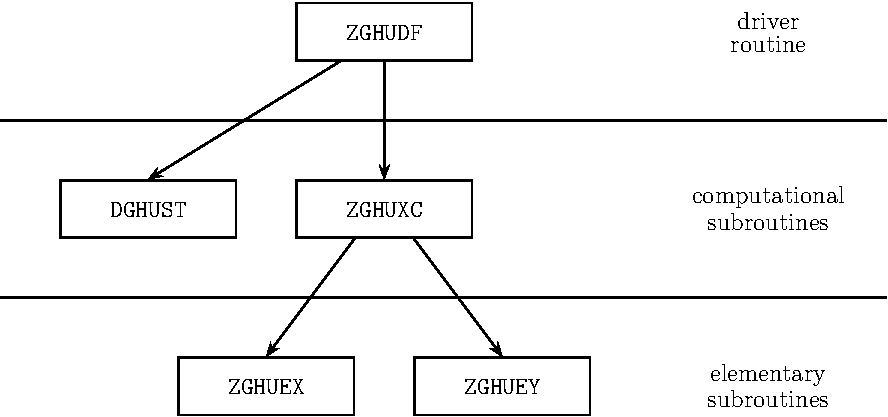
\includegraphics[width=0.8\textwidth]{complex_unfactored.pdf}
 \caption{Call graph of ZGHUDF.}
\end{figure}
%
\end{document}
